\documentclass{beamer}

\input{../Haust2015glærur}

\title{Tölvunarfræði 1a}
\subtitle{Vika 12, fyrri fyrirlestur}

\begin{document}

\begin{frame}
\titlepage
\end{frame}

\section{Inngangur}

\begin{frame}{Í síðasta þætti\ldots}
\begin{itemize}
 \item Stór verkefni (Ekki í kennslubók)
\end{itemize}
\end{frame}

\section{Teikning fyrir lengra komna (11.1)}

\begin{frame}{Teikniföll}
\begin{itemize}
 \item Höfum séð fallið \texttt{plot} til að teikna línurit áður
 \item Einnig:
 \begin{itemize}
  \item Föll til að merkja línuritin:
  \begin{itemize}
   \item \texttt{xlabel}, \texttt{ylabel}, \texttt{title}, \texttt{legend}
  \end{itemize}
  \item Fall til að kvarða ásana
  \begin{itemize}
   \item \texttt{axis}
  \end{itemize}
  \item Skipanir til að stýra teikningu
  \begin{itemize}
   \item \texttt{grid}, \texttt{hold}
  \end{itemize}
 \end{itemize}
\end{itemize}
\end{frame}

\begin{frame}[fragile]{Upprifjun um plot}
\begin{columns}
\column{0.50\textwidth}
\begin{minted}[fontsize=\small]{matlab}
>> x = linspace(-10,10);
>> y = sin(x).*x;
>> plot(x,y,'r*--')
>> axis([-10 10 -12 12])
>> title('Fallið f(x) = sin(x)*x')
>> grid on
\end{minted}
\column{0.50\textwidth}
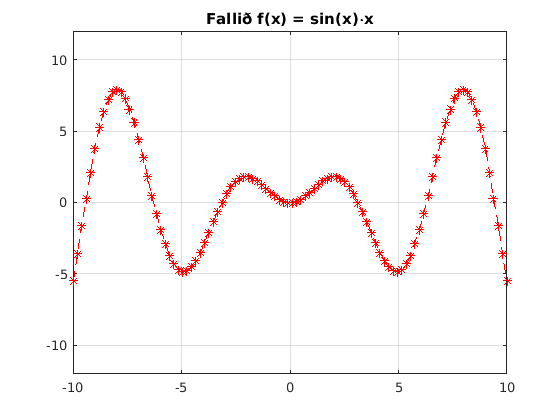
\includegraphics[width=\linewidth]{Pics/sintimesx}
\end{columns}
\end{frame}

\begin{frame}{Nýtt trix: Fylki línurita}
\begin{columns}
\column{0.6\textwidth}
\begin{itemize}
 \item Getum búið til fylki af línuritum með \texttt{subplot} fallinu
 \item Almennt form: \texttt{subplot(r, c, n)}
 \begin{itemize}
  \item Býr til $r \times c$ grind af línuritum
  \item $n$ táknar staðsetningu línuritsins í grindinni, í röð eftir línum
 \end{itemize}
\end{itemize}
\column{0.4\textwidth}
\begin{center}
Númer línuritanna í $2 \times 2$ grind af línuritum

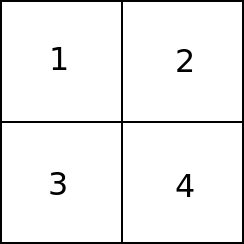
\includegraphics[width=0.8\linewidth]{Pics/subplotgrid}
\end{center}
\end{columns}
\end{frame}

\begin{frame}[fragile]{Dæmi}
\begin{columns}
\column{0.5\textwidth}
\begin{minted}[frame=lines, fontsize=\small]{matlab}
x = -2*pi:0.1:2*pi;
y = sin(x);
subplot(2,1,1);
plot(x,y);
xlabel('x');
ylabel('sin(x)');
axis([-2*pi 2*pi -1 1]);

y = cos(x);
subplot(2,1,2);
plot(x,y);
xlabel('x');
ylabel('cos(x)');
axis([-2*pi 2*pi -1 1]);
\end{minted}
\column{0.5\textwidth}
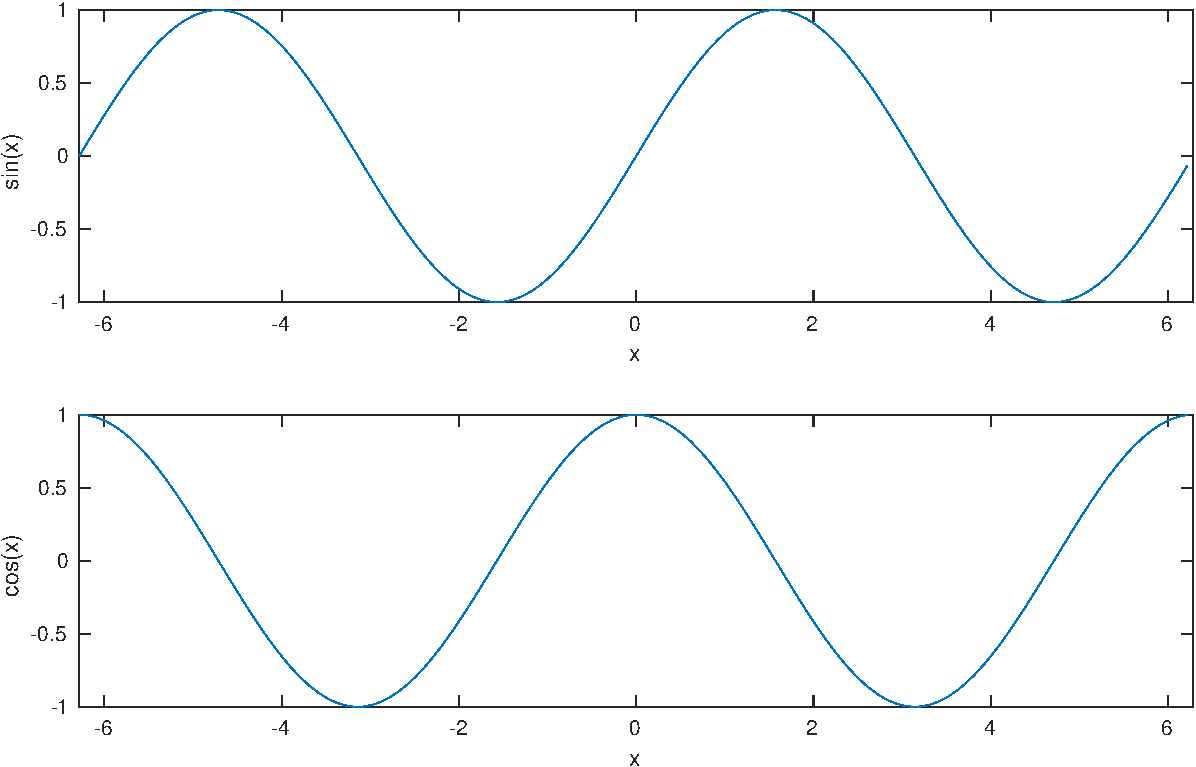
\includegraphics[width=\textwidth]{Pics/subplot-example.pdf}
\end{columns}
\end{frame}

\begin{frame}{Fleiri föll}
\begin{itemize}
 \item Hægt er að setja gögn fram á fleiri vegu en með \texttt{plot}
 \item Eftirfarandi föll vinna á nokkurn veginn sama hátt (en niðurstöðurnar líta mismunandi út)
 \begin{itemize}
  \item \texttt{plot} gerir línurit
  \item \texttt{bar} gerir súlurit
  \item \texttt{area} fyllir undir ferli
  \item \texttt{stem} gerir stofnteikningu
 \end{itemize}
\end{itemize}
\end{frame}

\begin{frame}{Dæmi}
\vspace{1cm}
Skoðum \texttt{subplottypes.m} á bls. 349. Það býr til

\begin{center}
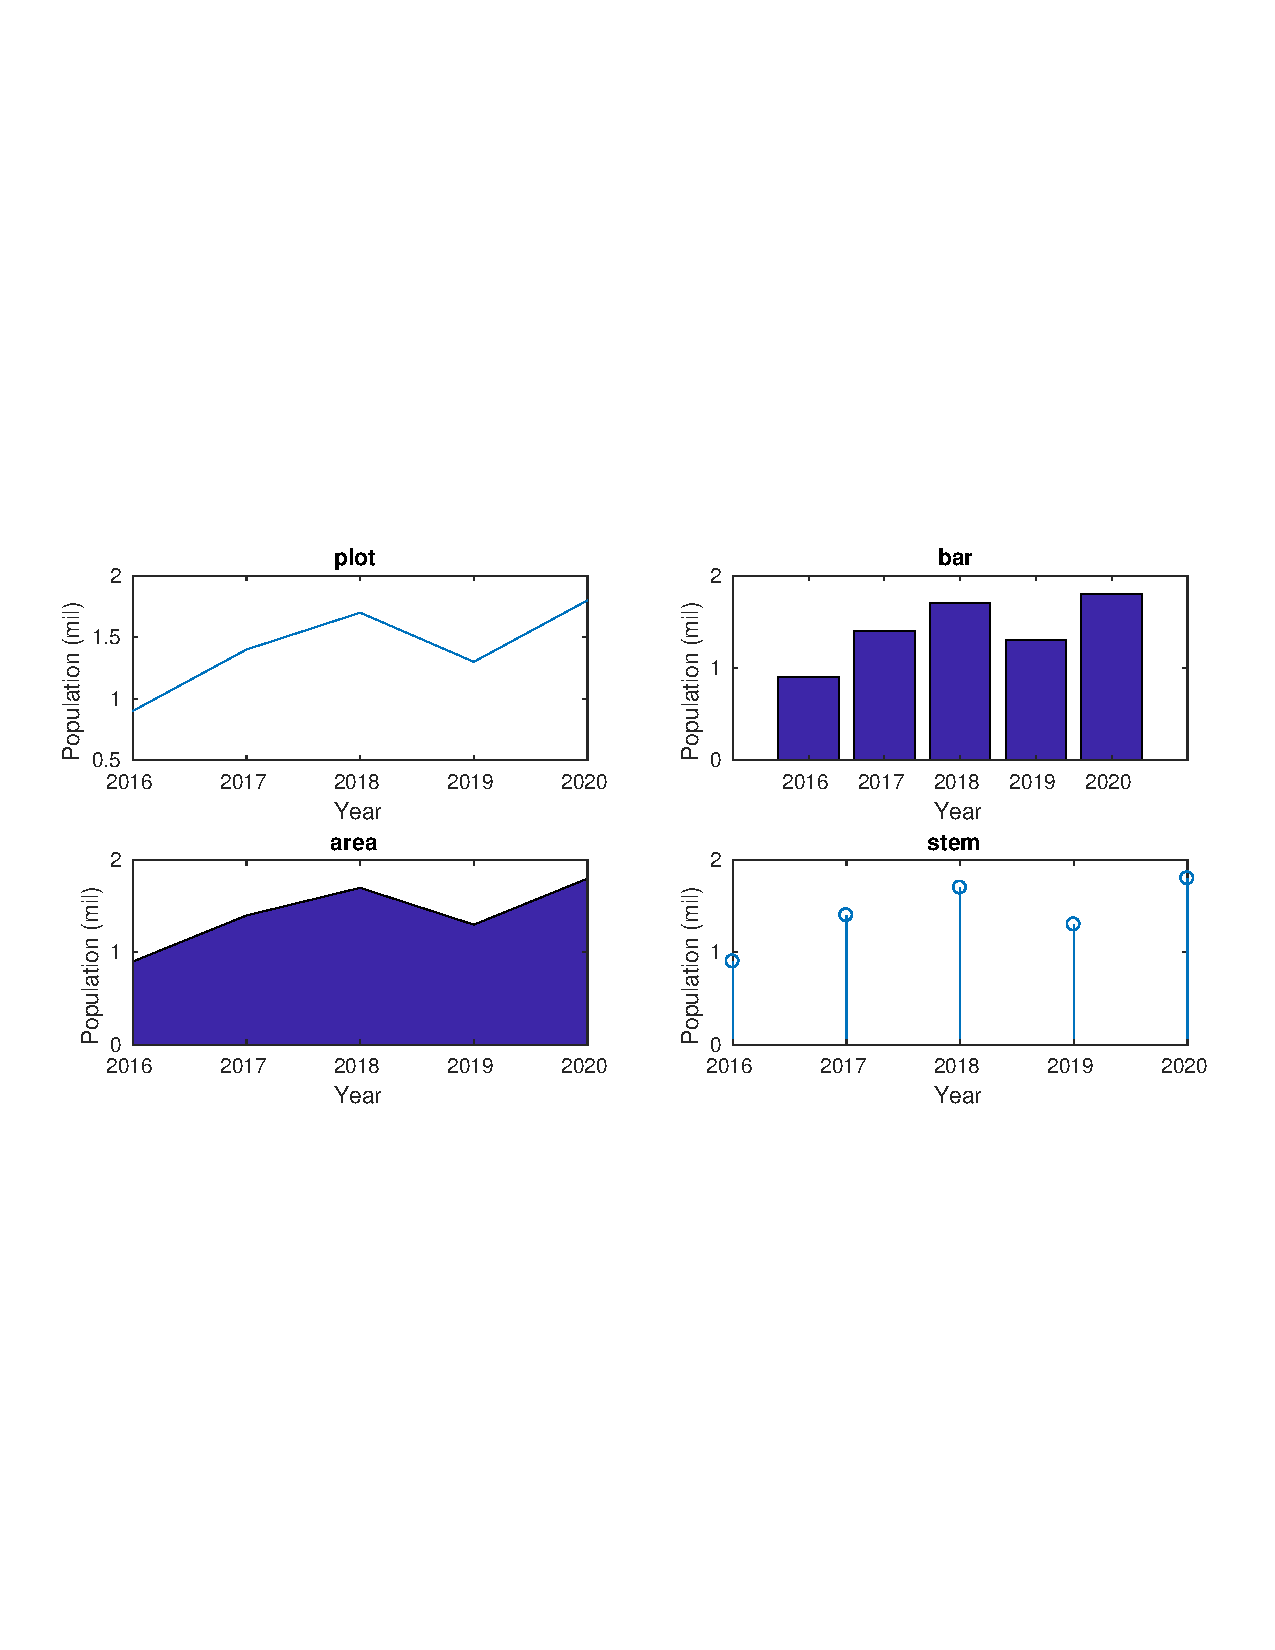
\includegraphics[width=0.6\textwidth]{Pics/plottypes.pdf}
\end{center}
\end{frame}

\subsection{Aðrar gerðir grafa}

\begin{frame}[fragile]{Tíðnirit}
Tíðnirit er súlurit sem sýnir hversu oft einstök gildi koma fyrir
\begin{columns}
\column{0.5\textwidth}
\begin{minted}[fontsize=\small]{matlab}
>> eink = [4 6 3 7 10 7 5 9 6 7];
>> hist(eink,1:10)
>> xlabel('Einkunn')
>> ylabel('Fjöldi')
\end{minted}

\column{0.5\textwidth}
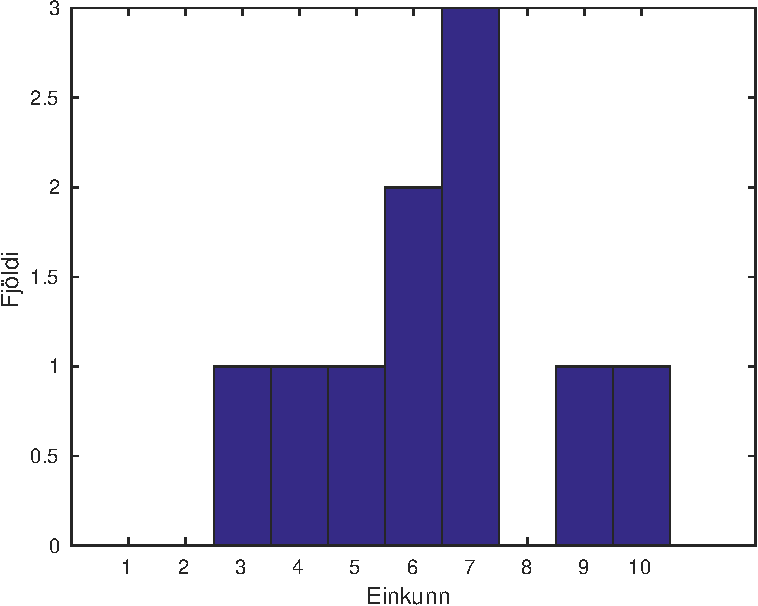
\includegraphics[width=\linewidth]{Pics/hist}
\end{columns}

\end{frame}

\begin{frame}[fragile]{Kökurit}
\vspace{1cm}
Kökurit sýnir gildi í vigri sem hlutfall af summu stakanna
\begin{columns}
\column{0.5\textwidth}
\begin{minted}[fontsize=\small]{matlab}
>> gildi = [11 14 8 3 1];
>> pie(gildi);
\end{minted}

\column{0.5\textwidth}
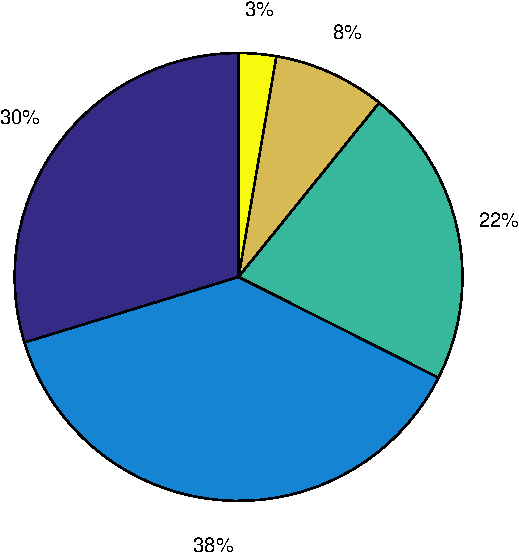
\includegraphics[width=\linewidth]{Pics/pie}
\end{columns}

\end{frame}

\begin{frame}[fragile]{Kökurit}
\vspace{1.5cm}
Getum látið kökurit vera með aðrar merkingar en prósentur (sjálfgefnar)
\begin{columns}
\column{0.5\textwidth}
\vspace{-0.5cm}
\begin{minted}[fontsize=\small]{matlab}
>> nofn = {'A','B','C','D','E'};
>> gildi = [11 14 8 3 1];
>> pie(gildi, nofn);
\end{minted}

\column{0.5\textwidth}
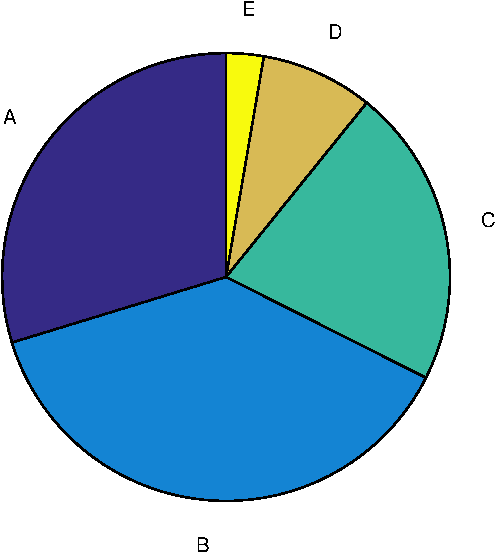
\includegraphics[width=\linewidth]{Pics/pie-names}
\end{columns}
\end{frame}

\section{Hreyfimyndir (11.2)}

\begin{frame}{Hreyfimyndir}
\begin{itemize}
 \item Fólk hefur gaman af því að sjá hreyfimyndir
 \item Tvær leiðir til að búa til hreyfimyndir í Matlab
 \begin{itemize}
  \item Rekja sig eftir teiknuðum ferli með \texttt{comet}
  \item Búa til ramma með \texttt{getframe} og sameina þá með \texttt{movie} fallinu
 \end{itemize}
\end{itemize}
\end{frame}

\begin{frame}[fragile]{Comet}
Notkun \texttt{comet} er mjög svipuð og notkun \texttt{plot}:
\begin{minted}{matlab}
>> x = -2*pi:0.01:2*pi;
>> y = sin(x);
>> comet(x,y)
\end{minted}
\end{frame}

\begin{frame}[fragile]{Movie}

Dæmigerð notkun \texttt{movie} er eftirfarandi:
\begin{verbatim}
for i=1:n
   teikniskipanir
   F(i) = getframe;
end
movie(F);
\end{verbatim}
Mörgum römmum er raðað inn í vigur, sem eru svo settir saman. Dæmi má sjá á bls. 355.

\end{frame}

\begin{frame}{Fyrirlestraræfing}
\begin{enumerate}
 \setcounter{enumi}{0}
 \item Teiknið föllin $\sin(x)$, $\cos(x)$ og $\tan(x)$ á bilinu $-\pi$ til $\pi$ hlið við hlið með \texttt{subplot}
 \item Í síðustu Alþingiskosningum fengu Sjálfstæðisflokkurinn (D) og Framsóknarflokkurinn (B) 19 þingmenn hvor, Samfylkingin (S) 9 þingmenn, Vinstri grænir (V) 7 þingmenn, Björt framtíð (A) 6 þingmenn og Píratar (Þ) 3 þingmenn. Sýnið þessa niðurstöðu í kökuriti með listabókstaf hvers flokks við hverja sneið.
 \item Teiknið upp fallið $x\cdot \cos(x)$ á bilinu $0$ til $20\pi$ með comet
\end{enumerate}
\end{frame}

\section{Óvissubil (utan bókar)}

\begin{frame}[fragile]{Að teikna með óvissubilum}
\begin{columns}
\column{0.55\textwidth}
Matlab er getur teiknað gagnapunkta með óvissubilum. Notum til þess \texttt{errorbar} fallið
\begin{minted}[fontsize=\small]{matlab}
>> x = 1:6;
>> y = [1 1.4 1.9 2.6 3 3.6];
>> e = [0.09 0.1 0.1 0.1 0.09 0.1];
>> errorbar(x,y,e)
\end{minted}
Lengd óvissubils númer $i$ er $2\cdot e(i)$.
\column{0.45\textwidth}
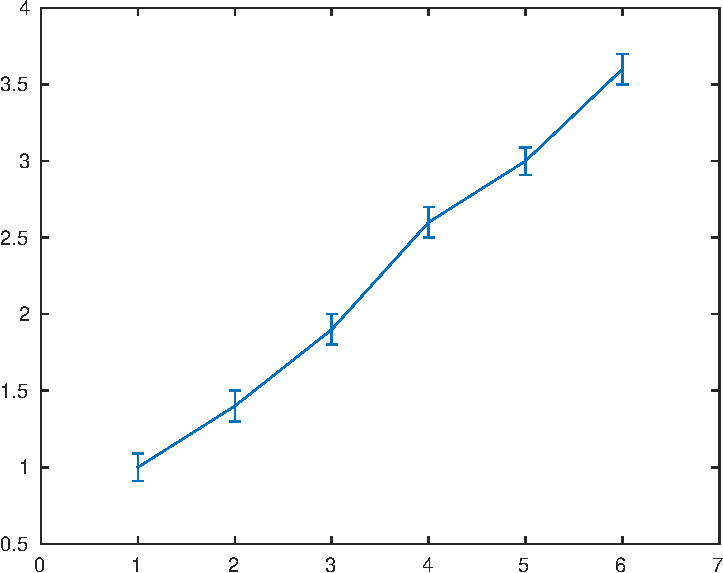
\includegraphics[width=\textwidth]{Pics/simple-errorbar}
\end{columns}
\end{frame}

\begin{frame}[fragile]{Mislöng óvissubil}
\begin{columns}
\column{0.55\textwidth}
Hægt er að láta efri og neðri óvissu vera mismikla með \texttt{errorbar}
\begin{minted}[fontsize=\scriptsize]{matlab}
>> x = 1:6;
>> y = [1 1.4 1.9 2.6 3 3.6];
>> l = [0.04 0.05 0.04 0.06 0.05 0.05];
>> u = [0.05 0.05 0.06 0.04 0.04 0.05];
>> errorbar(x,y,l,u)
\end{minted}
\column{0.45\textwidth}
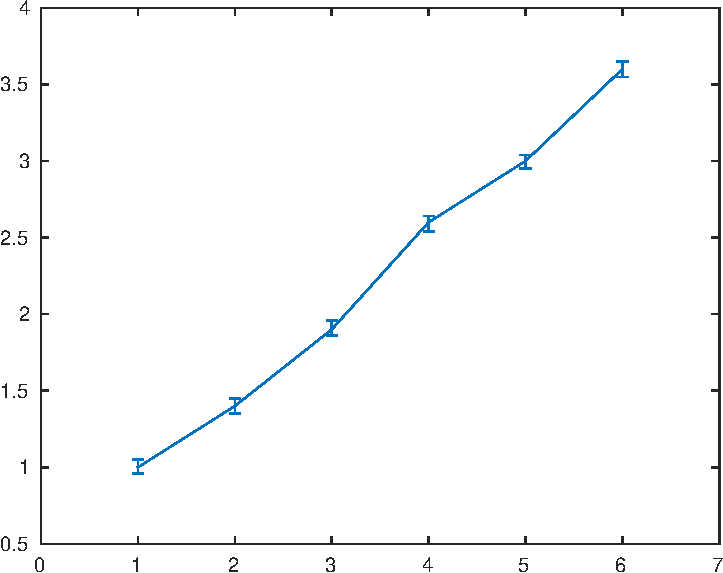
\includegraphics[width=\textwidth]{Pics/uneven-errorbar}
\end{columns}
\end{frame}

\begin{frame}{Óvissa á $x$-ás}
\begin{itemize}
 \item \texttt{errorbar} eins og það kemur úr kassanum ræður ekki við að teikna lárétt óvissubil
 \begin{itemize}
  \item Óheppilegt í verklegri eðlisfræði
 \end{itemize}
 \item Sem betur fer er Matlab forritunarmál, svo lausnir hafa fundist
 \begin{itemize}
  \item \href{http://www.mathworks.com/matlabcentral/fileexchange/40221-plot-data-with-error-bars-on-both-x-and-y-axes}{errorbarxy.m} - teiknar lárétt og lóðrétt óvissubil samtímis
  \item \href{http://www.mathworks.com/matlabcentral/fileexchange/3963-herrorbar}{herrorbar} - teiknar lárétt óvissubil (mætti nota með \texttt{hold on})
 \end{itemize}
\end{itemize}
\end{frame}

\section{Þrívíddarteikningar (11.3)}

\begin{frame}[fragile]{Þrívíddarteikningar}
\begin{columns}
\column{0.6\textwidth}
\begin{itemize}
 \item Matlab hefur nokkur föll fyrir þrívíddarteikningar
 \begin{itemize}
  \item Flest föllin eru eins og tvívíddarföll með ``3'' aftast
  \item Stundum fáum við bara upphleypta útgáfu af tvívíddarfallinu
 \end{itemize}
\end{itemize}
\begin{minted}{matlab}
>> gildi = [11 14 8 3 1];
>> pie3(gildi)
\end{minted}

\column{0.4\textwidth}
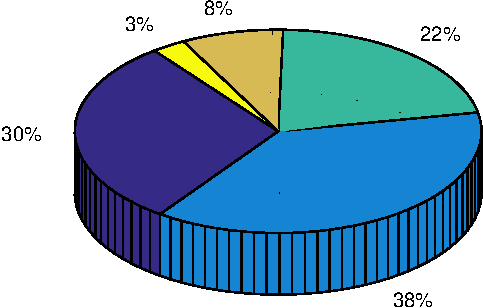
\includegraphics[width=\linewidth]{Pics/3dpie}
\end{columns}
\end{frame}

\begin{frame}[fragile]{Þrívíð súlurit}
\begin{columns}
\column{0.6\textwidth}
\begin{minted}{matlab}
>> ar = 2007:2011;
>> magn = [22 19 17 25 28];
>> bar3(ar,magn)
\end{minted}
\column{0.4\textwidth}
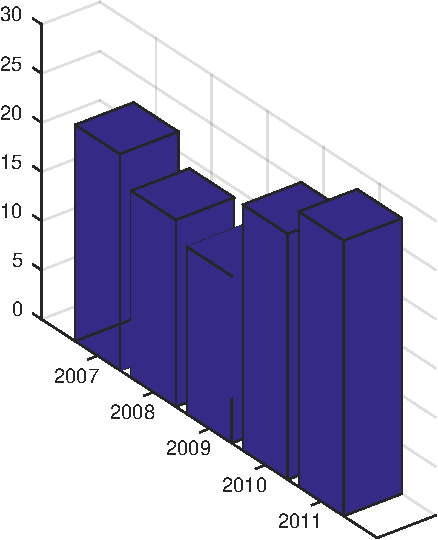
\includegraphics[width=\linewidth]{Pics/3dbar}
\end{columns}
\end{frame}

\begin{frame}[fragile]{Þrívíð súlurit}
\begin{columns}
\column{0.6\textwidth}
\begin{minted}{matlab}
>> m = randi([4 8], 3, 3);
>> bar3(m)
\end{minted}
\column{0.4\textwidth}
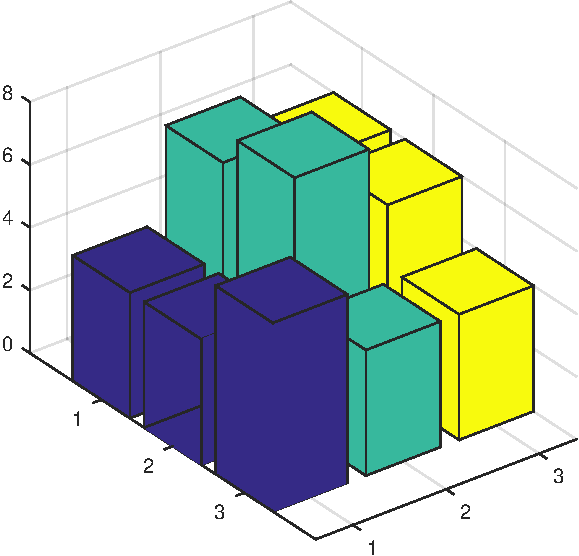
\includegraphics[width=\linewidth]{Pics/3dbar-matrix}
\end{columns}
\end{frame}

\begin{frame}[fragile]{Þrívíð línurit}
\begin{columns}
\column{0.6\textwidth}
Föllin \texttt{plot3} og \texttt{stem3} búa til ``alvöru'' þrívíddarteikningar út frá $x$, $y$ og $z$ vigrum
\begin{minted}{matlab}
>> t = 0:0.1:50;
>> plot3(sin(t),cos(t),t)
\end{minted}
\texttt{comet3} er líka til
\column{0.4\textwidth}
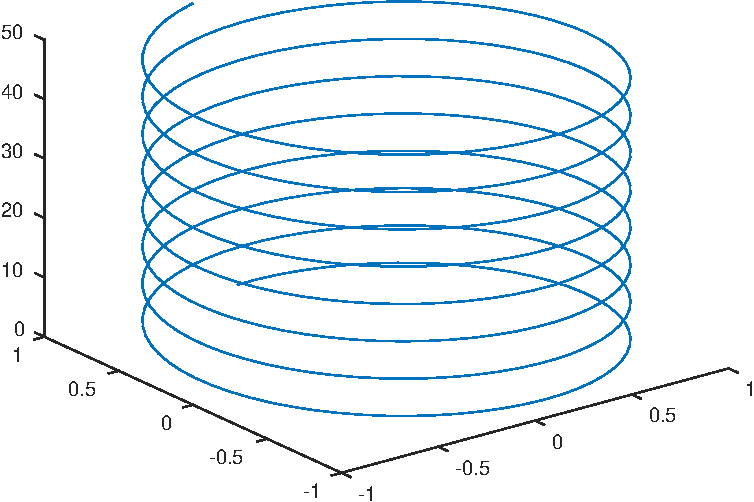
\includegraphics[width=\linewidth]{Pics/3dplot}
\end{columns}
\end{frame}

\subsection{Yfirborðsteikningar}

\begin{frame}{Yfirborðsteikningar}
\begin{itemize}
 \item Föllin \texttt{mesh} og \texttt{surf} búa til þrívíddarmyndir af yfirborðum
 \item Taka við þremur viðföngum
 \begin{itemize}
  \item Fylki af \texttt{x}-hnitum
  \item Fylki af \texttt{y}-hnitum
  \item Fylki af \texttt{z}-hnitum (hæð yfir $xy$-sléttunni)
 \end{itemize}
\end{itemize}
\end{frame}

\begin{frame}[fragile]{Dæmi um \texttt{mesh}}
\vspace{1cm}
Teiknum upp fallið $xe^{-x^2-y^2}$
\begin{minted}{matlab}
>> [x y] = meshgrid(-2:0.2:2, -1.5:0.2:1.5);
>> z = x.*exp(-x.^2 - y.^2);
>> mesh(x,y,z)
\end{minted}

\begin{center}
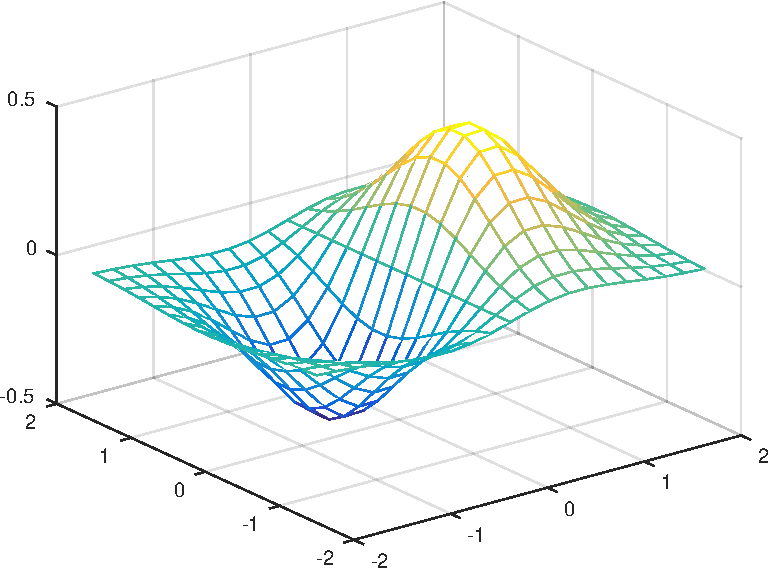
\includegraphics[width=0.4\linewidth]{Pics/3dmesh}
\end{center}
\end{frame}

\begin{frame}[fragile]{Að smíða hnitakerfi}
\begin{itemize}
 \item \texttt{meshgrid} fallið er mikið notað til að búa til fylki til þrívíddarteikningar
 \begin{itemize}
  \item Það afritar inntaksvigra svo úr verði fylki
  \item Fallsgildin eru síðan reiknuð út frá fylkjunum
 \end{itemize}
 \item Fleiri föll eru til til að smíða punkta
 \begin{itemize}
  \item \texttt{sphere} býr til kúlu
 \end{itemize}
\end{itemize}
\begin{minted}{matlab}
>> [x, y, z] = sphere(10);
>> mesh(x, y, z)
\end{minted}
\end{frame}

\begin{frame}{surf og shading}
\begin{itemize}
 \item \texttt{surf} fallið virkar eins og \texttt{mesh}, en með fyllingu á milli ``möskvanna''
 \item \texttt{shading} stillir það hvernig yfirborðið er litað
 \begin{itemize}
  \item \texttt{shading faceted} er sjálfgefið, býr til flata litun með línur á köntum
  \item \texttt{shading flat} býr til flata litun án kanta
  \item \texttt{shading interp} brúar (e. \emph{interpolates}) litina á milli flata
 \end{itemize}
\end{itemize}
\end{frame}

\begin{frame}{Fyrirlestraræfing}
\begin{columns}
\column{0.6\textwidth}
\begin{enumerate}
 \setcounter{enumi}{3}
 \item Notið \texttt{errorbar} til að teikna mynd af gögnunum til hliðar, með gefinni óvissu á $y$-ásnum
 \item Teiknið fallið
 \[
 \frac{\sin(\sqrt{x^2 + y^2})}{\sqrt{x^2 + y^2}}
 \]
 á bilinu $-6\pi$ til $6\pi$ fyrir $x$ og $y$
\end{enumerate}
\column{0.4\textwidth}
\begin{tabular}{lll}
\toprule
$x$&$y$&óvissa\\
\midrule
1&1.1&0.15\\
2&2.0&0.25\\
3&2.9&0.20\\
4&3.7&0.40\\
5&5.0&0.10\\
\bottomrule
\end{tabular}
\end{columns}
\end{frame}



\end{document}
